%
% $RCSfile: hierarchy_and_ontology.tex,v $
%
% Copyright (c) 2001-2004. Christian Heller. All rights reserved.
%
% No copying, altering, distribution or any other actions concerning this
% document, except after explicit permission by the author!
% At some later point in time, this document is planned to be put under
% the GNU FDL license. For now, _everything_ is _restricted_ by the author.
%
% http://www.cybop.net
% - Cybernetics Oriented Programming -
%
% http://www.resmedicinae.org
% - Information in Medicine -
%
% @author Christian Heller <christian.heller@tuxtax.de>
%

\section{Hierarchy and Ontology}
\label{hierarchy_and_ontology_heading}

Section \ref{basic_patterns_heading} explained three design patterns that are
widely used in software architectures. It has shown similarities between them
and raised the question if they could possibly be merged into just one pattern,
called \emph{Translator}, what will be described in section
\ref{logical_architecture_heading}.
Yet before, this section will demonstrate how the principle of \emph{Hierarchy}
may be applied to obtain an \emph{Ontology}.

%
% $RCSfile: association_elimination.tex,v $
%
% Copyright (C) 2002-2008. Christian Heller.
%
% Permission is granted to copy, distribute and/or modify this document
% under the terms of the GNU Free Documentation License, Version 1.1 or
% any later version published by the Free Software Foundation; with no
% Invariant Sections, with no Front-Cover Texts and with no Back-Cover
% Texts. A copy of the license is included in the section entitled
% "GNU Free Documentation License".
%
% http://www.cybop.net
% - Cybernetics Oriented Programming -
%
% http://www.resmedicinae.org
% - Information in Medicine -
%
% Version: $Revision: 1.1 $ $Date: 2008-08-19 20:41:05 $ $Author: christian $
% Authors: Christian Heller <christian.heller@tuxtax.de>
%

\subsection{Association Elimination}
\label{association_elimination_heading}
\index{Association Elimination}
\index{Hierarchy as Principle}
\index{Ontology}
\index{Electronic Health Record}
\index{EHR}
\index{Episode Based EHR}
\index{Object Oriented Programming}
\index{OOP}
\index{Super Model}
\index{Sub Model}
\index{Granularity of Items}
\index{Unidirectional Dependency}
\index{Eliminated Sub Associations}
\index{Ontological Level}
\index{Layers of a System}
\index{Top-most Super Category}

To pursue the idea of a purely hierarchical software system, it seems useful to
investigate in which way domain data models can get simplified. This section
therefore demonstrates how the principle of \emph{Hierarchy} may be applied to
obtain an \emph{Ontology} \cite{hellerkunze}.

\begin{figure}[ht]
    \begin{center}
        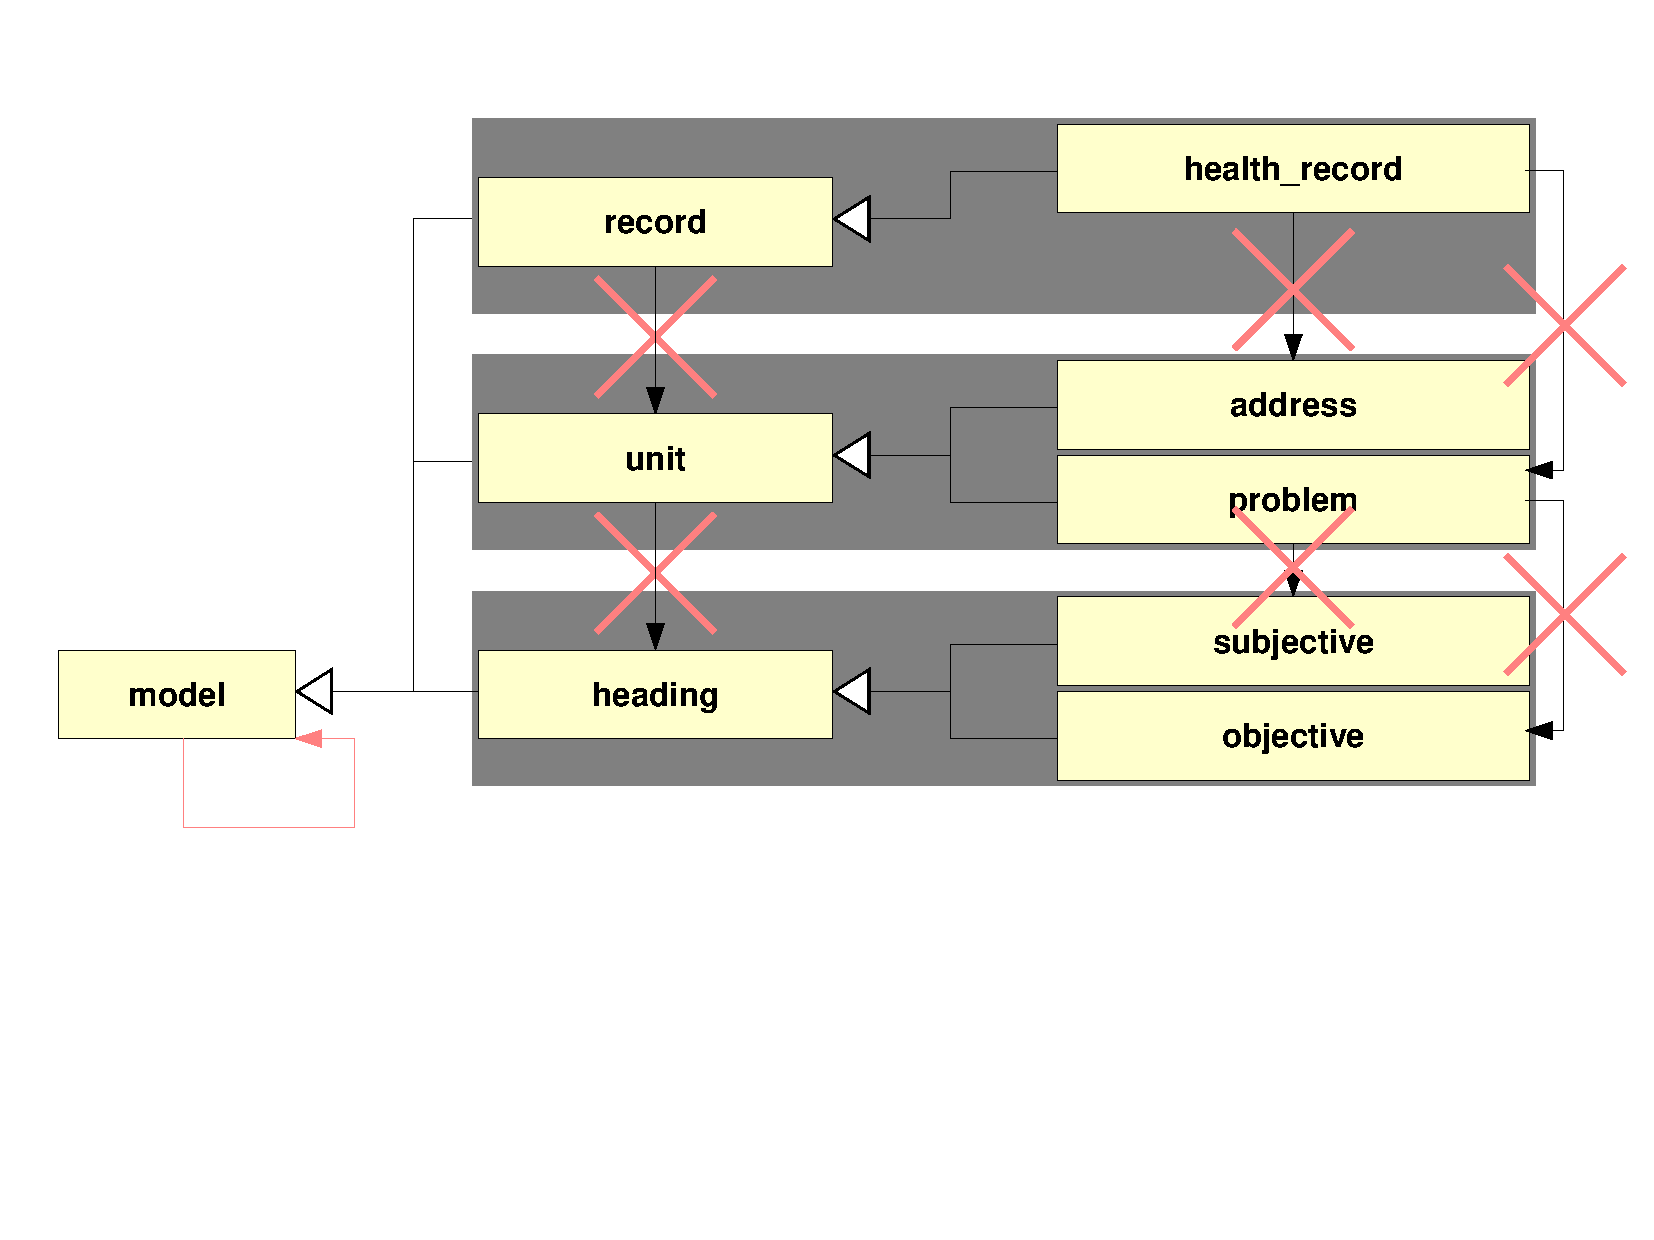
\includegraphics[scale=0.3,angle=-90]{graphic/elimination.pdf}
        \caption{Association Elimination in an EHR}
        \label{elimination_figure}
    \end{center}
\end{figure}

An \emph{Electronic Health Record} (EHR) will serve as example domain model,
whose simplified structure is shown in figure \ref{elimination_figure}. It
consists of numerous parts whereof two may be \emph{Address} and \emph{Problem}.
Following the \emph{Episode-based EHR} recommendation \cite{westerhof},
\emph{Problem} may, besides others, consist of parts of type \emph{Subjective}
and \emph{Objective}. All these associations between part models are needed to
navigate through the overall domain model.

A frequent design decision in classical \emph{Object Oriented Programming}
(OOP) is to sum up common properties of \emph{Sub} models by introducing a
\emph{Super} model (category). It should never be \emph{Properties}, but rather
the \emph{Granularity} of objects leading to the creation of a super category,
as the later section \ref{categorisation_versus_composition_heading} will
recommend. The \emph{OpenEHR} project \cite{openehr} suggests to let the
above-mentioned sub models inherit from the more coarse-grained super
categories \emph{Record}, \emph{Unit} and \emph{Heading}.

Whichever reason -- once the super categories are there, they should be
associated similarly to their sub categories, that is in the same direction,
using solely \emph{unidirectional} dependencies. (The problematic nature of
bidirectional dependencies was elaborated in section \ref{pattern_heading}.)
Afterwards, all associations between sub categories become superfluous as every
sub category can reach its sibling across the super categories' association
(figure \ref{elimination_figure}). In other words:
\emph{Super- eliminate Sub Associations}.

Here a short Java code example for how the \emph{HealthRecord} may retrieve a
reference to \emph{Address}:

\begin{scriptsize}
    \begin{verbatim}
    Address a = (Address) get_element("address");
    \end{verbatim}
\end{scriptsize}

\emph{HealthRecord} inherits the \emph{get\_element} method from its super
category \emph{Record}. \emph{Record} holds differing sub models of category
\emph{Unit} and other instances. The \emph{get\_element} method delivers back
a general \emph{Model} that still needs to be down-casted to the expected sub
category \emph{Address}.

\begin{figure}[ht]
    \begin{center}
        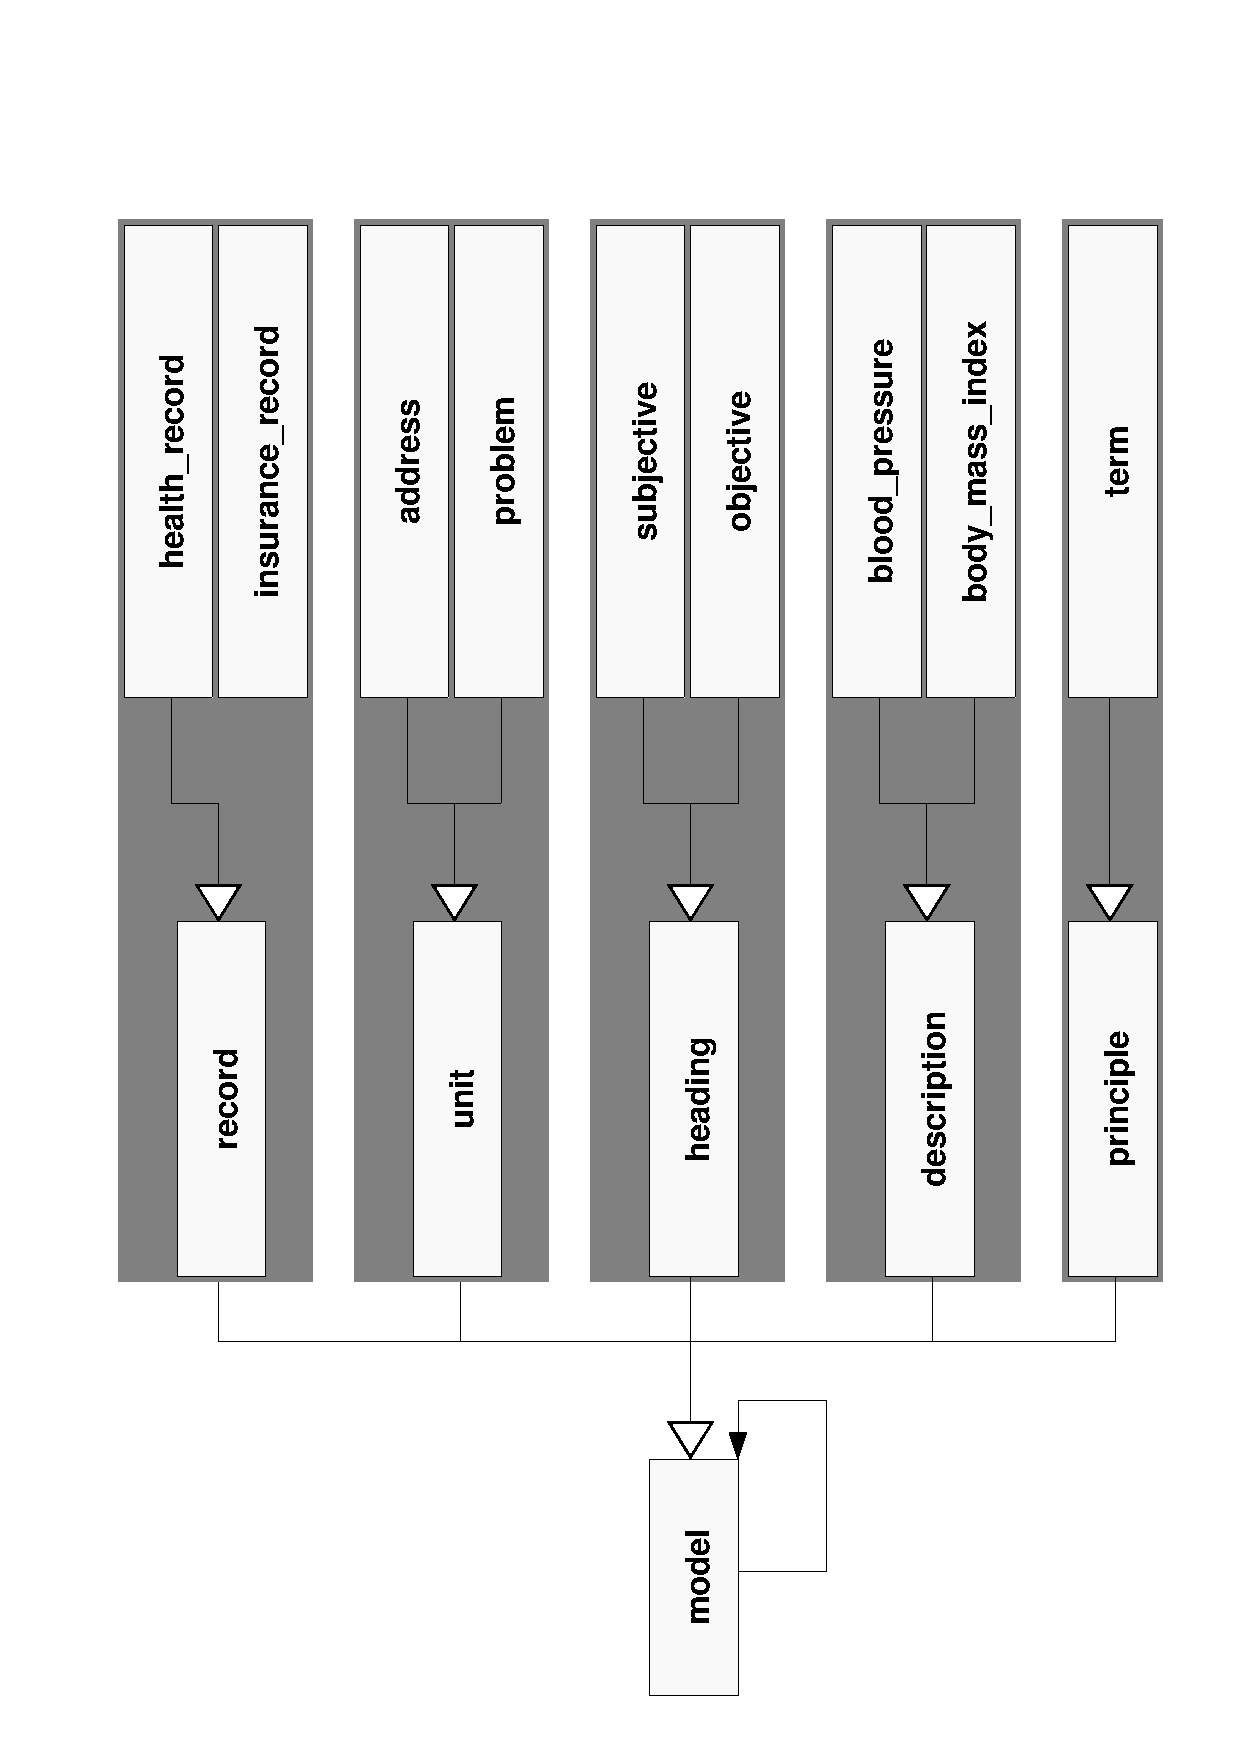
\includegraphics[scale=0.3,angle=-90]{graphic/levels.pdf}
        \caption{Model Container and Ontological Levels}
        \label{levels_figure}
    \end{center}
\end{figure}

The definition of models, their dependencies (defined by associations) and
granularities (defined by inheritance) in a software system results in several
\emph{Layers} of models of common granularity (figure \ref{levels_figure}).
These layers are often called \emph{Ontological Level} as they, together, form
an \emph{Ontology} (sections \ref{ontology_heading},
\ref{knowledge_ontology_heading}).

An ontology of that kind can, of course, be created for every knowledge model.
The financial sector -- like an insurance company, for example -- may use an
\emph{Insurance Record} with comparable structure.

The idea to structure software as a system of \emph{Layers} was also suggested
by the equally named pattern in section \ref{layers_heading}. The difference
between the two is that the \emph{Layers} pattern divides a system only by its
\emph{Functionality}, for example into \emph{User Interface}, \emph{Domain},
\emph{Data Mapper} and \emph{Data Source}. An \emph{Ontology} additionally
groups model items by their \emph{Granularity}. By inheriting from a common
superior category, sub categories indicate that they logically belong to the
same \emph{Layer}.

Continuing the structuring process of introducing more and more common super
categories, for all equally-granular items, the development culminates in one
top-most super category of all other categories in the system, which this paper
calls \emph{Model}. It is as general as the \emph{java.lang.Object} class for
the Java class library \cite{java}, only that it additionally represents a
\emph{Container} that can store models of any category, as explained in
\cite{hellerbohl}. In other words, \emph{Model} provides the meta functionality
of a container behaviour to \emph{all} other categories in a system.

%
% $RCSfile: ontology.tex,v $
%
% Copyright (c) 2001-2004. Christian Heller. All rights reserved.
%
% No copying, altering, distribution or any other actions concerning this
% document, except after explicit permission by the author!
% At some later point in time, this document is planned to be put under
% the GNU FDL license. For now, _everything_ is _restricted_ by the author.
%
% http://www.cybop.net
% - Cybernetics Oriented Programming -
%
% http://www.resmedicinae.org
% - Information in Medicine -
%
% @author Christian Heller <christian.heller@tuxtax.de>
%

\subsection{Ontology}
\label{ontology_heading}

Manifold definitions of the word \emph{Ontology} exist. They come from philosophy,
metaphysics, information technology and others -- too many to list here.
This document uses its own, adapted definition and considers an ontology to be
\emph{a strict hierarchy of abstract items, organized in levels of growing
granularity, that are solely unidirectionally related}. It such represents a
systematic description of complex domain contexts.

\begin{figure}[ht]
    \begin{center}
        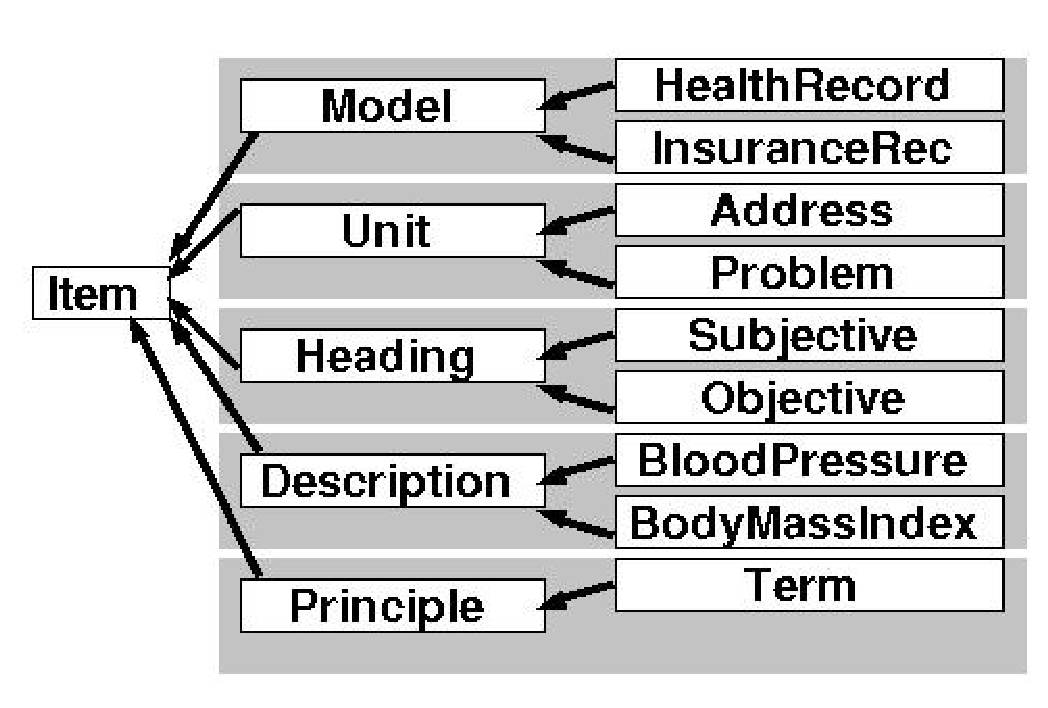
\includegraphics[scale=0.4]{vector/electronic_health_record_ontology.eps}
        \caption{Electronic Health Record Ontology}
        \label{electronic_health_record_ontology_figure}
    \end{center}
\end{figure}

Figure \ref{electronic_health_record_ontology_figure} shows one possible ontology
of an electronic health record, as described in the previous section.



